%%
%% Alex Ihler
%%
\documentclass[twoside,11pt]{article}
\usepackage{amsmath,amsfonts,amssymb,amsthm}
\usepackage{graphicx,color}
\usepackage{verbatim,url}
\usepackage{listings}
\usepackage{upquote}
\usepackage[T1]{fontenc}
%\usepackage{lmodern}
\usepackage[scaled]{beramono}
%\usepackage{textcomp}
\usepackage{ifthen}

% Directories for other source files and images
\newcommand{\bibtexdir}{../bib}
\newcommand{\figdir}{eps}

\newcommand{\E}{\mathrm{E}}
\newcommand{\Var}{\mathrm{Var}}
\newcommand{\N}{\mathcal{N}}
\newcommand{\matlab}{{\sc Matlab}\ }

\setlength{\textheight}{9in} \setlength{\textwidth}{6.5in}
\setlength{\oddsidemargin}{-.25in}  % Centers text.
\setlength{\evensidemargin}{-.25in} %
\setlength{\topmargin}{0in} %
\setlength{\headheight}{0in} %
\setlength{\headsep}{0in} %

\renewcommand{\labelenumi}{(\alph{enumi})}
\renewcommand{\labelenumii}{(\arabic{enumii})}

\theoremstyle{definition}
\newtheorem{MatEx}{M{\scriptsize{ATLAB}} Usage Example}

\definecolor{comments}{rgb}{0,.5,0}
\definecolor{backgnd}{rgb}{.95,.95,.95}
\definecolor{string}{rgb}{.2,.2,.2}
\lstset{language=Matlab}
\lstset{basicstyle=\small\ttfamily,
        mathescape=true,
        emptylines=1, showlines=true,
        backgroundcolor=\color{backgnd},
        commentstyle=\color{comments}\ttfamily, %\rmfamily,
        morecomment=[l]{\%},
        morecomment=[is]{\%\#}{\%\#},
        stringstyle=\color{string}\ttfamily,
        keywordstyle=\ttfamily, %\normalfont,
        showstringspaces=false}
\newcommand{\matp}{\mathbf{\gg}}

\newcommand{\myraise}{\vspace{-.15cm}}

\newcommand{\problem}[3]{
 \begin{minipage}{\textwidth}
 \noindent{\large {\bf Problem #1:} #2}
 #3
 \end{minipage}
 \vspace{2\baselineskip}
}

\begin{document}

\centerline{\Large {\bf Your Name: } CS74/174 Homework \#1}
\centerline{Machine Learning and Statistical Data Analysis: Winter 2016}
\vspace{1cm}

\subsection*{Problem 0: Getting Connected}
Please join our class forum on Piazza, \\
\url{https://piazza.com/dartmouth/winter2016/cosc07401cosc17401wi16/home}\\
Please post your questions and discussion points on Piazza, rather than by email
to me or the TA, since chances are that other students have the same or similar questions,
and will be helped by seeing the discussion.  


\subsection*{Problem 1: Matlab \& Data Exploration}
\begin{enumerate}
\item Download and load the ``Fisher iris'' data set into Matlab (or Octave):
\begin{lstlisting}
 iris=load('data/iris.txt');     % load the text file
 y = iris(:,end);           % target value is last column
 X = iris(:,1:end-1);       % features are other columns
 whos                       % show current variables in memory and sizes
\end{lstlisting}
The Iris data consist of four real-valued features used to predict which of three types of iris
flower was measured (a three-class classification problem).
\item Use \texttt{size(X,2)} to get the number of features, and \texttt{size(X,1)} to get 
the number of data points.
\item The histogram (``\texttt{hist}'') of the data is shown in Figure~\ref{fig:hist_plot}.  
\item Compute the mean of the data points for each feature (\texttt{mean})
\item  The standard KNN is based on Euclidean distance $d(x^{(1)},x^{(2)}) = \sqrt{\sum_i (x_i^{(1)}-x_i^{(2)})^2}$. 
\begin{align}
y & = [y^{(1)}, \ldots, y^{(n)}]\\
X & = [x^{(1)}, \cdots, x^{(n)}] 
\end{align}
$$
x^{(1)} = [x^{(1)}_1, \ldots, x^{(1)}_d]
$$

$$
X = \begin{bmatrix}
x^{(1)}_1& x^{(1)}_2  & x^{(1)}_3 \\
x^{(2)}_1& x^{(2)}_2 & x^{(2)}_3 \\
x^{(3)}_1& x^{(3)}_2 & x^{(3)}_3 \\
x^{(4)}_1& x^{(4)}_2 & x^{(4)}_3 
\end{bmatrix}
$$
\end{enumerate}

\begin{figure}[htbp]
   \centering
   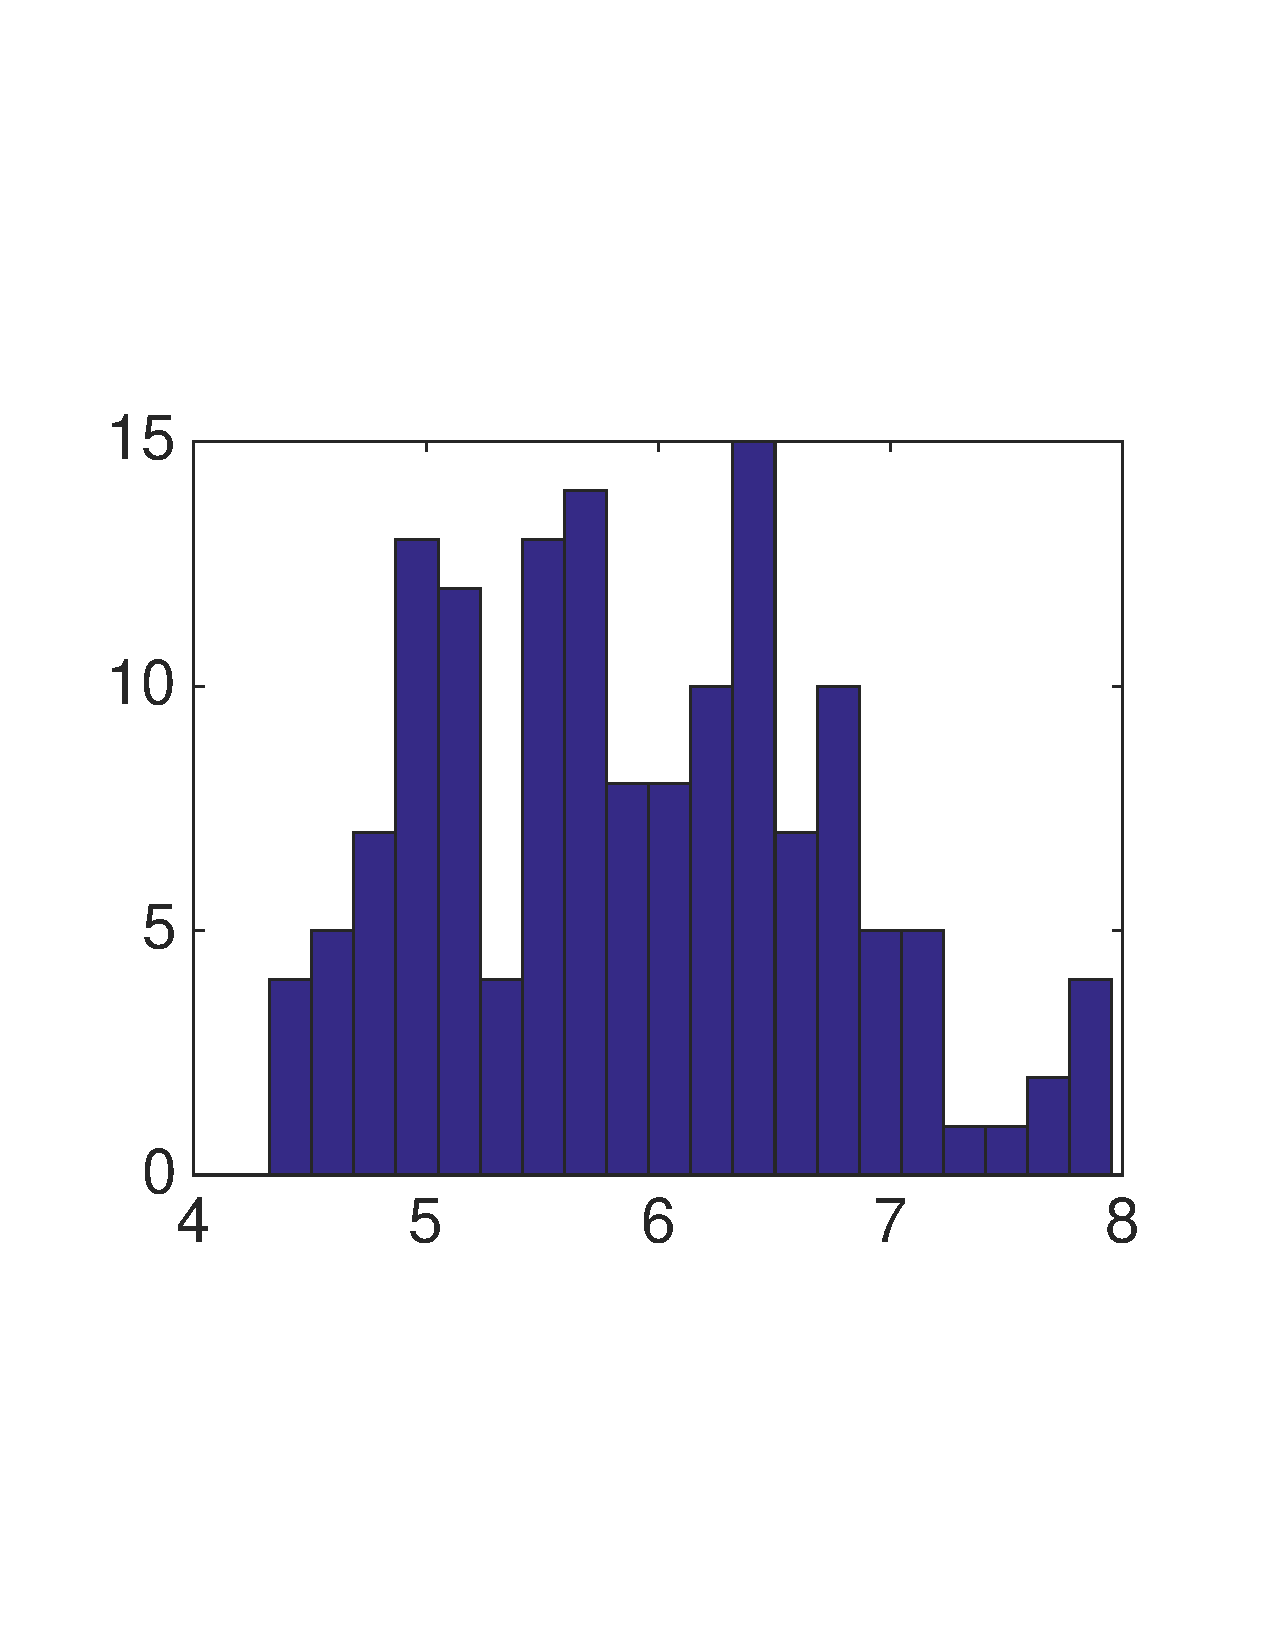
\includegraphics[width = .5\textwidth]{figures/hist_iris.pdf} % requires the graphicx package
   \caption{\textbf{Problem 1(c)}: The histogram of Iris data (the first feature)}
   \label{fig:hist_plot}
\end{figure}


\end{document}
